\documentclass[a4paper,12pt]{article}
% \input{../../../config.tex}
\usepackage{../../../mypackages}
\usepackage{../../../macros}


\usepackage{pgfplots}
    \pgfplotsset{
    compat=1.11,
  }

\usetikzlibrary{shapes,arrows,babel}
\tikzstyle{box}=[minimum size = 0.1cm, rectangle, draw=black, fill=gray]
% Define the global variable

% Function that meets the requirements + ways to do custom drawing
% https://tex.stackexchange.com/questions/490374/a-curve-pass-via-points-at-tikz


\def\WITH_CORRECTION{YES}


\begin{document}

\title{Fonctions - Rappels de 2nde}
\author{N. Bancel}

\sloppy  % This will apply the sloppy setting to the entire document.
\maketitle

\section{Vocabulaire des fonctions - Fonctions affines}

\begin{enumerate}
  \item A chaque nombre réel \(x\) d'un intervalle \(I\), une fonction \(f\) associe un nombre réel et un seul que l'on note \(f(x)\). Qu'est ce qu'une image ? Qu'est-ce que l'ensemble de définition ? Qu'est qu'un antécédent ? \par
  \ans{
    \begin{minipage}{0.5\textwidth}
    \begin{itemize}
      \item[$\bullet$] \(f(x)\) est \textbf{l'image} de \(x\) par la fonction \(f\)
      \item[$\bullet$] \(I\) est \textbf{l'ensemble de définition} de \(f\)
      \item[$\bullet$] Lorsque \(y = f(x)\), on dit que le nombre \(x\) est un \textbf{antécédent} du nombre \(y\) par la fonction \(f\)
    \end{itemize}
    \end{minipage}%
    \begin{minipage}{0.5\textwidth}
    \centering
    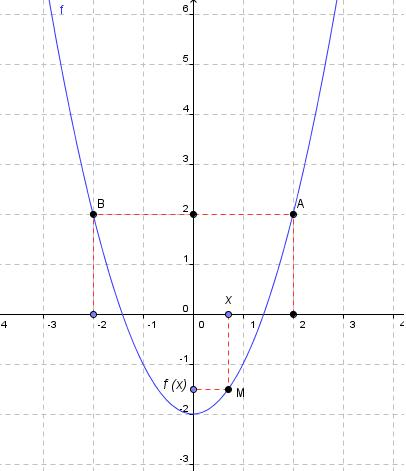
\includegraphics[width=0.5\textwidth]{image_antecedent.jpg}
    \end{minipage}
    Dans la figure ci-dessus : 
    \begin{itemize}
      \item[$\bullet$] Si M a pour abscisse \(x\), alors son ordonnée est \(f(x)\).
      \item[$\bullet$] A a pour coordonnées (2 ; 2), donc \(f(2) = 2\), donc \textbf{l’image de 2 par \(f\) est 2}.
      \item[$\bullet$] B a pour coordonnées (-2 ; 2), donc \(f(-2) = 2\) donc \textbf{l’image de -2 par \(f\) est 2}.
      \item[$\bullet$] Les \textbf{antécédents} de 2 par la fonction f sont -2 et 2.
    \end{itemize}
    }{6}{FALSE}
  \item Quelle est l'expression d'une fonction affine ? Quelle est la représentation graphique d'une fonction affine ? \par
    \ans{
      Une fonction affine est une fonction définie sur \(\mathbb{R}\) par \(f(x) = ax + b\) où  \(a\) et \(b\) désignent deux nombres réels donnés. \par
      Sa représentation graphique est une \textbf{droite} \par
      \begin{tcolorbox}
      \textbf{Vocabulaire} : Dans un repère, \(d\) est la droite représentant une fonction affine \( f : x \mapsto ax + b \)
      \begin{itemize}
        \item[$\bullet$] \textcolor{red}{a} est le \textcolor{red}{coefficient directeur} de \(d\)
        \item[$\bullet$] \textcolor{blue}{b} est \textcolor{blue}{l'ordonnée à l'origine} de \(d\) (ordonnée du point d'intersection de \(d\) avec l'axe des ordonnées)
      \end{itemize}
      \end{tcolorbox}
      \begin{minipage}{0.5\textwidth}
        \centering
        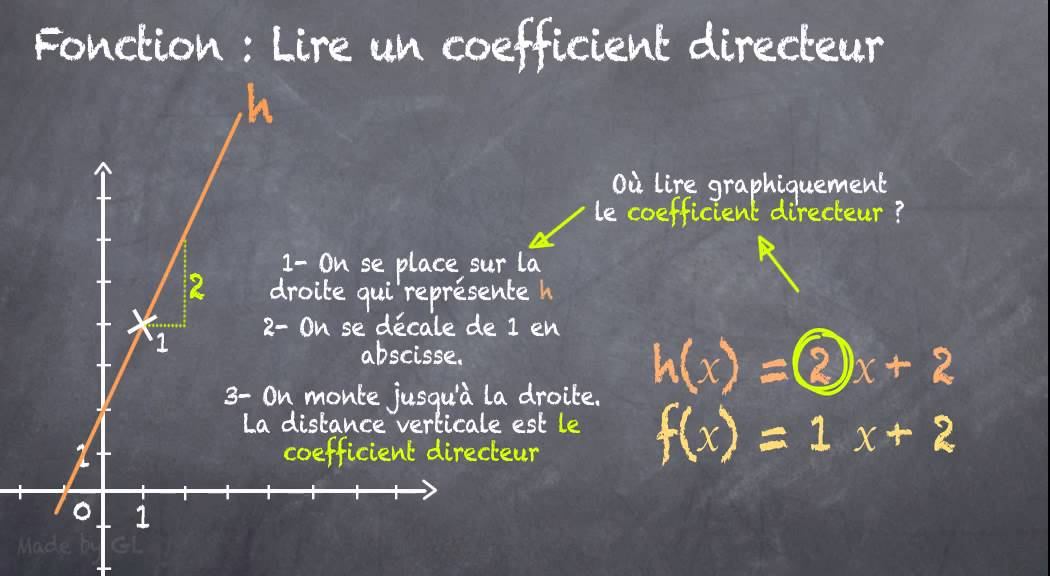
\includegraphics[width=\textwidth]{coef_directeur.jpg}
        \captionof{figure}{Source : \href{https://www.youtube.com/watch?v=ni1cSNtLgWY}{Fonction : Lire un coefficient directeur}}
      \end{minipage}
      \begin{minipage}{0.5\textwidth}
        \centering
        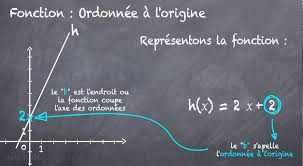
\includegraphics[width=\textwidth]{ordonnée à l'origine.jpeg}
        \captionof{figure}{Source : \href{https://www.youtube.com/watch?v=iX6LklqqPXI}{Fonction : Ordonnée à l'origine}}
      \end{minipage}
    }{4}{FALSE}
\end{enumerate}

\section{Les fonctions de référence}

\begin{enumerate}
  \item Quelle est l'expression de la fonction \textbf{carré} ? Quelle est sa propriété principale (en terme de symétrie) ? \par
  \ans{
    La fonction carré est la fonction \(f\) définie sur \(\mathbb{R}\) par \textbf{\(f(x) = x^2\)} \par 
    La représentation graphique de la fonction carré est appelée \textbf{parabole} \par
    Elle est \textbf{symétrique par rapport à l'axe des ordonées}
    \begin{figure}[H]
      \centering
      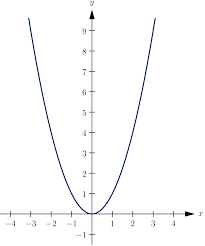
\includegraphics[width=0.3\linewidth]{carré.png}
      \caption{\label{} La fonction carré}
  \end{figure}
  }{4}{FALSE}
  \item Quelle est l'expression de la fonction \textbf{inverse} ? Quelle est sa propriété principale (en terme de symétrie) ? \par
  \ans{
    La fonction inverse est la fonction \(f\) définie sur \(\mathbb{R^*}\) par \textbf{\(f(x) = 1/x\)} \par 
    La représentation graphique de la fonction inverse est appelée \textbf{hyperbole} \par
    Elle est \textbf{symétrique par rapport à l'origine O du repère}
    \begin{figure}[H]
      \centering
      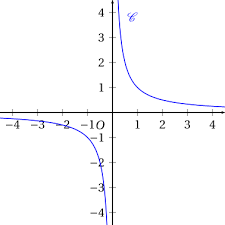
\includegraphics[width=0.3\linewidth]{inverse.png}
      \caption{\label{} La fonction inverse}
  \end{figure}
  }{4}{FALSE}
  \item Quelle est l'expression de la fonction \textbf{cube} ? Quelle est sa propriété principale (en terme de symétrie) ? \par
  \ans{
    La fonction cube est la fonction \(f\) définie sur \(\mathbb{R}\) par \textbf{\(f(x) = x^3\)} \par 
    La représentation graphique de la fonction cube est \textbf{symétrique par rapport à l'origine O du repère}
    \begin{figure}[H]
      \centering
      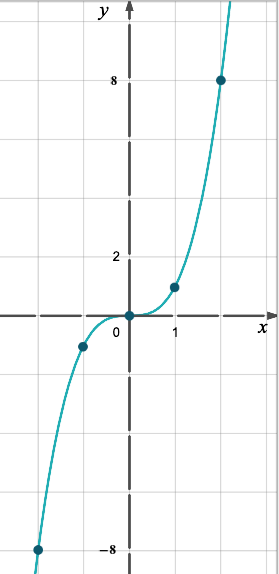
\includegraphics[width=0.25\linewidth]{cube.png}
      \caption{\label{} La fonction cube}
  \end{figure}
  }{4}{FALSE}
  \item Quelle est l'expression de la fonction \textbf{racine carrée} ? Quel est son intervalle de définition ? \par
  \ans{
    La fonction racine carrée est la fonction \(f\) définie sur l'intervalle \([0, +\infty[\). par \textbf{\(f(x) = \sqrt(x)\)} \par 
    \begin{figure}[H]
      \centering
      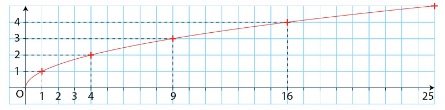
\includegraphics[width=\linewidth]{racine_carree.jpg}
      \caption{\label{} La fonction racine carrée}
  \end{figure}
  }{4}{FALSE}
\end{enumerate}

\section{Courbes représentatives des fonctions}

\begin{enumerate}
  \item A partir du graphique ci-dessous, résoudre graphiquement l'équation \(f(x) = k\) \par
  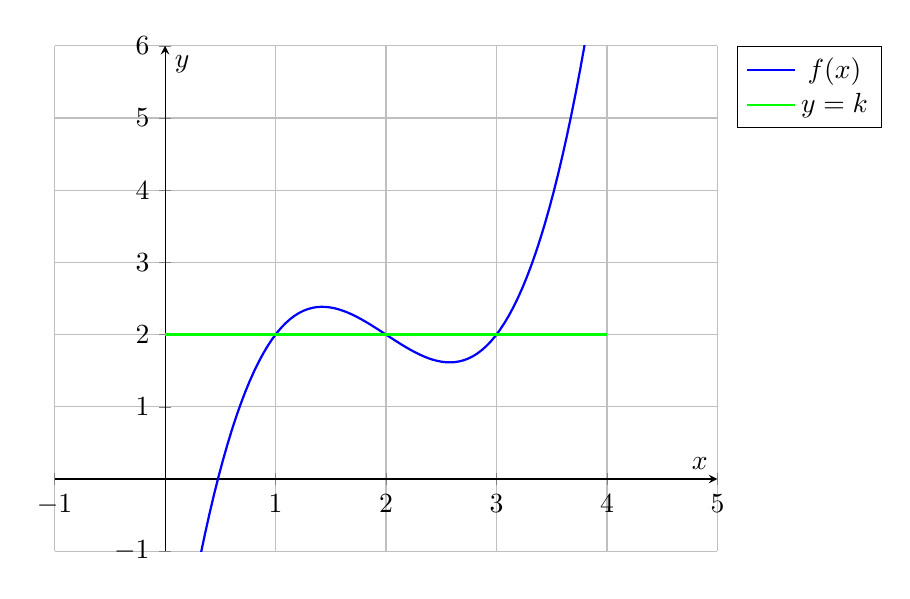
\begin{tikzpicture}
    \begin{axis}[
        axis lines = middle,
        xlabel = $x$,
        ylabel = {$y$},
        xmin=-1, xmax=5,
        ymin=-1, ymax=6,
        domain=0:4,
        samples=100,
        legend pos=outer north east,
        grid=major,
        width=10cm, height=8cm,
    ]
    % Plot f(x) = (x-1)*(x-2)*(x-3) + 2
    \addplot[color=blue, thick] {(x-1)*(x-2)*(x-3) + 2};
    \addlegendentry{$f(x)$}
    
    % Plot y = k
    \addplot[color=green, thick] {2};
    \addlegendentry{$y = k$}
    \end{axis}
    \end{tikzpicture} \par 

  \ans{
    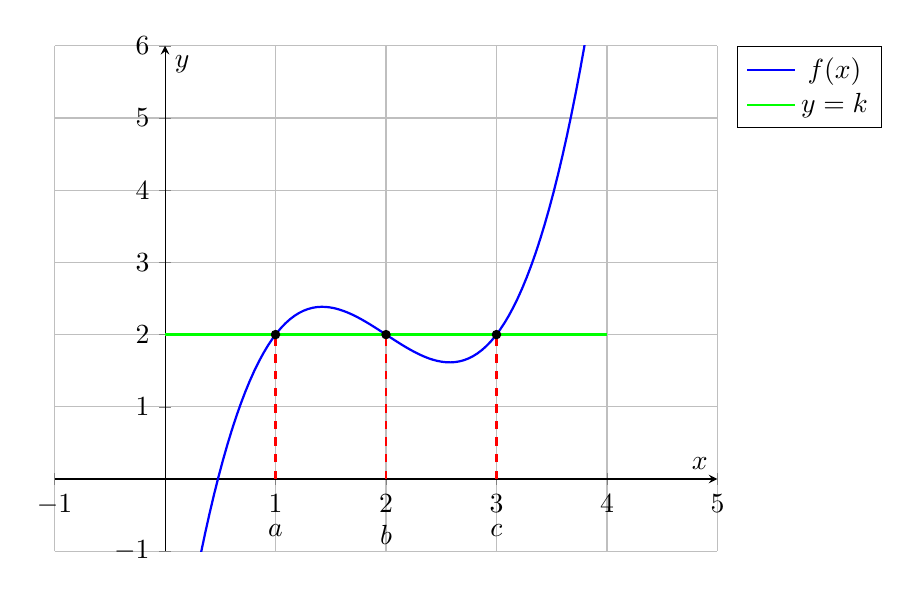
\begin{tikzpicture}
      \begin{axis}[
          axis lines = middle,
          xlabel = $x$,
          ylabel = {$y$},
          xmin=-1, xmax=5,
          ymin=-1, ymax=6,
          domain=0:4,
          samples=100,
          legend pos=outer north east,
          grid=major,
          width=10cm, height=8cm,
      ]
      % Plot f(x) = (x-1)*(x-2)*(x-3) + 2
      \addplot[color=blue, thick] {(x-1)*(x-2)*(x-3) + 2};
      \addlegendentry{$f(x)$}
      
      % Plot y = k
      \addplot[color=green, thick] {2};
      \addlegendentry{$y = k$}
      
      % Mark the solutions
      \addplot[mark=*, mark size=1.5pt, color=black] coordinates {(1, 2)};
      \addplot[mark=*, mark size=1.5pt, color=black] coordinates {(2, 2)};
      \addplot[mark=*, mark size=1.5pt, color=black] coordinates {(3, 2)};
  
      \addplot[red, dashed, thick]
              coordinates {(1, 0) (1, 2)};
      \addplot[red, dashed, thick]
              coordinates {(2, 0) (2, 2)};
      \addplot[red, dashed, thick]
              coordinates {(3, 0) (3, 2)};
      
      % Labels for the solutions
      \node at (axis cs: 1,-0.5) [anchor=north] {$a$};
      \node at (axis cs: 2,-0.5) [anchor=north] {$b$};
      \node at (axis cs: 3,-0.5) [anchor=north] {$c$};
      
      \end{axis}
      \end{tikzpicture} \par 
    Sur cette figure l'équation \(f(x) = k\) a pour solutions les nombres \textcolor{red}{a, b, et c}.
  }{6}{FALSE}
  \item A partir du graphique ci-dessous, résoudre graphiquement l'équation \(f(x) = g(x)\) \par
  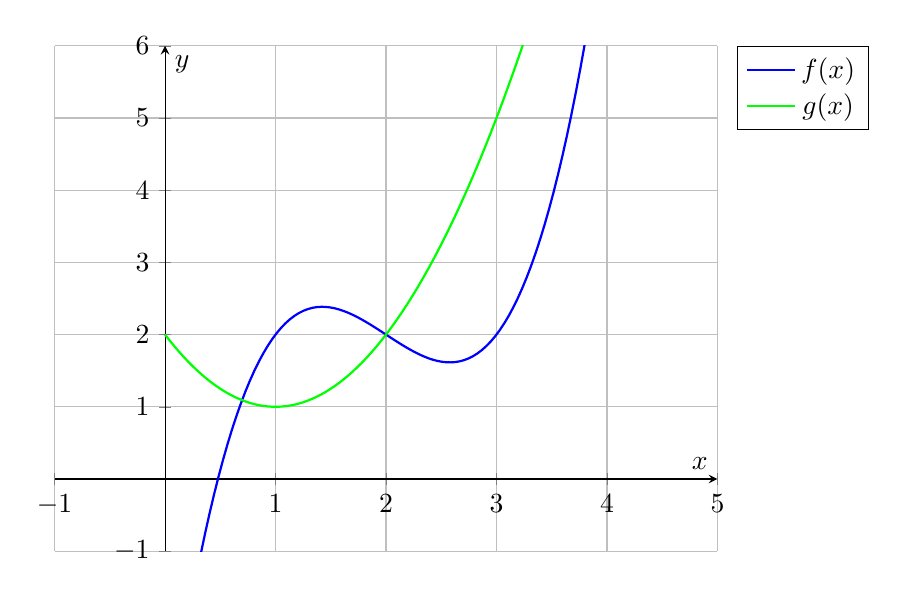
\begin{tikzpicture}
    \begin{axis}[
        axis lines = middle,
        xlabel = $x$,
        ylabel = {$y$},
        xmin=-1, xmax=5,
        ymin=-1, ymax=6,
        domain=0:4,
        samples=100,
        legend pos=outer north east,
        grid=major,
        width=10cm, height=8cm
        ]
    % Plot f(x) = (x-1)*(x-2)*(x-3) + 2
    \addplot[color=blue, thick] {(x-1)*(x-2)*(x-3) + 2};
    \addlegendentry{$f(x)$}
    
    % Plot y = k
    \addplot[color=green, thick] {(x-1)^2+1};
    \addlegendentry{$g(x)$}
    \end{axis}
  \end{tikzpicture} \par
  \ans{

  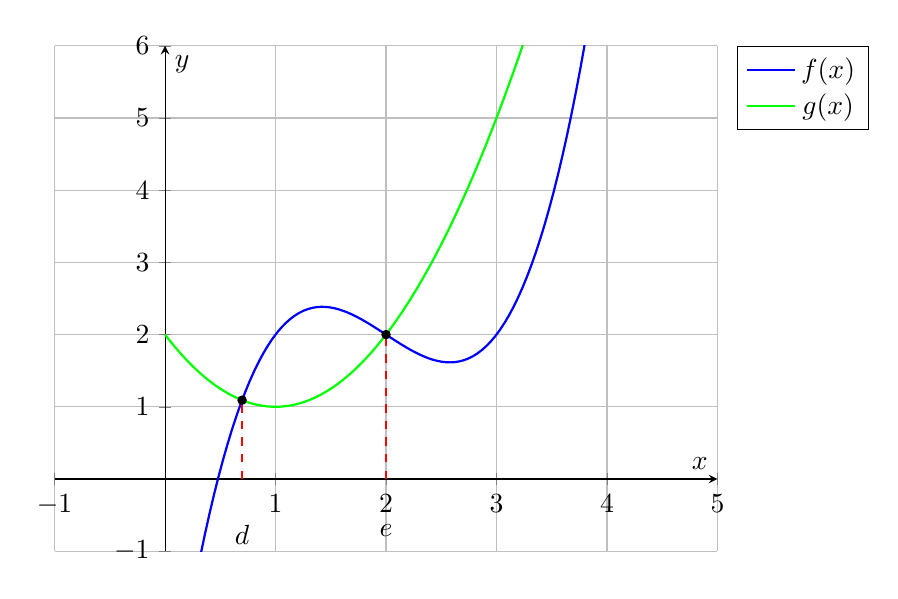
\begin{tikzpicture}
    \begin{axis}[
        axis lines = middle,
        xlabel = $x$,
        ylabel = {$y$},
        xmin=-1, xmax=5,
        ymin=-1, ymax=6,
        domain=0:4,
        samples=100,
        legend pos=outer north east,
        grid=major,
        width=10cm, height=8cm,
    ]
    % Plot f(x) = (x-1)*(x-2)*(x-3) + 2
    \addplot[color=blue, thick] {(x-1)*(x-2)*(x-3) + 2};
    \addlegendentry{$f(x)$}
    
    % Plot y = k
    \addplot[color=green, thick] {(x-1)^2+1};
    \addlegendentry{$g(x)$}
    
    % Mark the solutions
    \addplot[mark=*, mark size=1.5pt, color=black] coordinates {(0.6972, 1.091673)};
    \addplot[mark=*, mark size=1.5pt, color=black] coordinates {(2, 2)};

    \addplot[red, dashed, thick]
            coordinates {(0.6972, 0) (0.6972, 1.091673)};
    \addplot[red, dashed, thick]
            coordinates {(2, 0) (2, 2)};
    
    % Labels for the solutions
    \node at (axis cs: 0.6972,-0.5) [anchor=north] {$d$};
    \node at (axis cs: 2,-0.5) [anchor=north] {$e$};
    
    \end{axis}
\end{tikzpicture} \par
Sur cette figure l'équation \(f(x) = g(x)\) a pour solutions les nombres \textcolor{red}{d et e}.
  }{5}{FALSE}
\end{enumerate}

\section{Fonction paire / Fonction impaire}
\begin{enumerate}
  \item Qu'est-ce qu'une fonction paire ? \par
  
  \ans{
    
  \begin{minipage}{0.5\textwidth}
    \(f\) est définie sur un ensemble D. \(f\) est une fonction \textbf{paire} si 
  \begin{enumerate}
    \item[$\bullet$] Pour tout \(x\) de D, \(-x\) appartient aussi à D
    \item[$\bullet$] Pour tout \(x\) de D, \(f(-x)=f(x)\) appartient aussi à D
  \end{enumerate}
  \end{minipage}%
  \begin{minipage}{0.5\textwidth}
    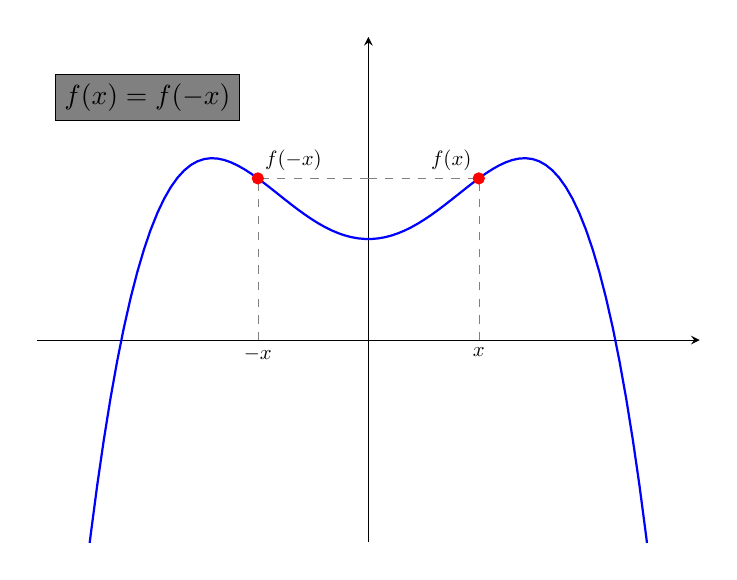
\begin{tikzpicture}
        \begin{axis}[
            axis lines = middle,
            xmin=-3, xmax=3,
            ymin=-10, ymax=15,
            domain=-3:3,
            samples=100,
            width=10cm, height=8cm,
            grid=none, % Supprime le quadrillage
            xtick style={draw=none}, % Enlève les graduations sur x
            ytick style={draw=none}, % Enlève les graduations sur x
            xticklabel=\empty, % enlève les 1, 2, 3 etc sur l'axe des y
            yticklabel=\empty % enlève les 1, 2, 3 etc sur l'axe des y
        ]
    
        % Définition de la fonction
        \addplot[color=blue, thick] {-x^4 + 4*x^2 + 5};
    
        %TO DO : try to parametrize the x1 and y1
        % f(-1) = 8
    
        %\pgfmathsetmacro{\x_1}{1}
        %\pgfmathsetmacro{\x_2}{-1}
        %\pgfmathsetmacro{\y_1}{-\x_1^4 + 4*\x_1^2 + 5}
        %\pgfmathsetmacro{\y_2}{-\x_2^4 + 4*\x_2^2 + 5}
    
        \addplot [color=red,mark=*] coordinates {(1,8)};
        \addplot [color=red,mark=*] coordinates {(-1,8)};
        \draw [dashed,help lines] (0,8) -- (1,8);
        \draw [dashed,help lines] (1,0) -- (1,8);
        \draw [dashed,help lines] (0,8) -- (-1,8);
        \draw [dashed,help lines] (-1,0) -- (-1,8);
    
        % scale makes f(x) smaller
    
        \draw (1,8) node[above left,scale=0.75]{$f(x)$}; 
        \draw (-1,8) node[above right,scale=0.75]{$f(-x)$};
        \draw (1,0) node[below,scale=0.75]{$x$};
        \draw (-1,0) node[below,scale=0.75]{$-x$};
        
        \node[box](f) at (-2,12) {$f(x) = f(-x)$};
        %\node[box](f) at (2,12) {$f(x) = f(-x)$};
        
    \end{axis}
    \end{tikzpicture}
  \end{minipage}%
  }{4}{FALSE}

  \item Qu'est-ce qu'une fonction impaire ? \par
  \ans{
  \begin{minipage}[b]{0.5\textwidth}
    \(f\) est définie sur un ensemble D. \(f\) est une fonction \textbf{impaire} si 
  \begin{enumerate}
    \item[$\bullet$] Pour tout \(x\) de D, \(-x\) appartient aussi à D
    \item[$\bullet$] Pour tout \(x\) de D, \(f(-x)=-f(x)\) appartient aussi à D
  \end{enumerate}
    \end{minipage}%
  \begin{minipage}{0.5\textwidth}
\tikzstyle{box}=[minimum size = 0.1cm, rectangle, draw=black, fill=gray]
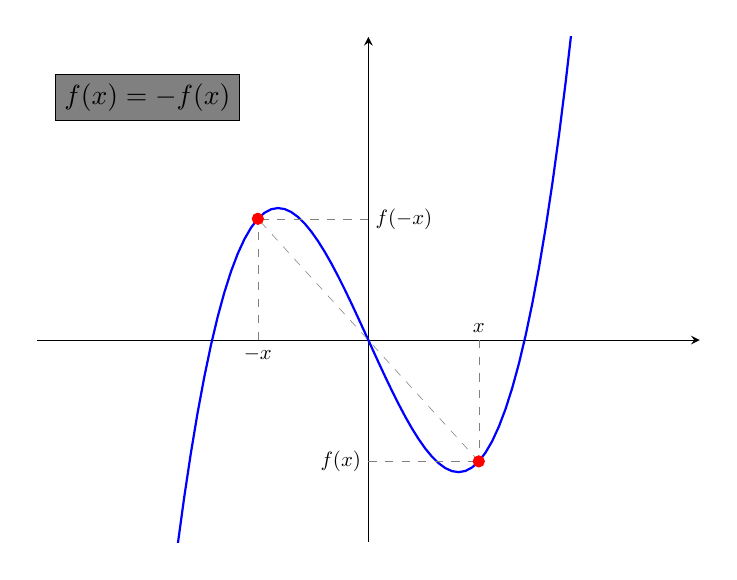
\begin{tikzpicture}
  \begin{axis}[
      axis lines = middle,
      xmin=-3, xmax=3,
      ymin=-10, ymax=15,
      domain=-3:3,
      samples=100,
      width=10cm, height=8cm,
      grid=none, % Supprime le quadrillage
      xtick style={draw=none}, % Enlève les graduations sur x
      ytick style={draw=none}, % Enlève les graduations sur x
      xticklabel=\empty, % enlève les 1, 2, 3 etc sur l'axe des y
      yticklabel=\empty % enlève les 1, 2, 3 etc sur l'axe des y
  ]

  % Définition de la fonction
  \addplot[color=blue, thick] {6*x*(x^2 - 2)};

  %TO DO : try to parametrize the x1 and y1
  % f(-1) = 8

  %\pgfmathsetmacro{\x_1}{1}
  %\pgfmathsetmacro{\x_2}{-1}
  %\pgfmathsetmacro{\y_1}{-\x_1^4 + 4*\x_1^2 + 5}
  %\pgfmathsetmacro{\y_2}{-\x_2^4 + 4*\x_2^2 + 5}

  \addplot [color=red,mark=*] coordinates {(-1,6)};
  \addplot [color=red,mark=*] coordinates {(1,-6)};
  \draw [dashed,help lines] (0,6) -- (-1,6); % Vertical left
  \draw [dashed,help lines] (-1,0) -- (-1,6); % Horizontal left
  \draw [dashed,help lines] (1,0) -- (1,-6);  % Vertical right
  \draw [dashed,help lines] (0,-6) -- (1,-6); % Horizontal right
  \draw [dashed,help lines] (1,-6) -- (-1,6); % Diagonal

  % scale makes f(x) smaller

  \draw (0,-6) node[left,scale=0.75]{$f(x)$}; 
  \draw (0,6) node[right,scale=0.75]{$f(-x)$};
  \draw (1,0) node[above,scale=0.75]{$x$};
  \draw (-1,0) node[below,scale=0.75]{$-x$};

  \node[box](f) at (-2,12) {$f(x) = - f(x)$};
  
\end{axis}
\end{tikzpicture}
\end{minipage}
}{4}{FALSE}
\end{enumerate} 

\section{Variations et extremums}

\begin{enumerate}
  \item Quelle est la définition d'une fonction croissante ? D'une fonction décroissante ? \par
  \begin{minipage}{0.37\textwidth}
    \begin{tikzpicture}
        \begin{axis}[
            axis lines = middle,
            xmin=-2, xmax=2,
            ymin=-10, ymax=15,
            domain=-3:3,
            samples=100,
            width=10cm, height=8cm,
            grid=none, % Supprime le quadrillage
            xtick style={draw=none}, % Enlève les graduations sur x
            ytick style={draw=none}, % Enlève les graduations sur x
            xticklabel=\empty, % enlève les 1, 2, 3 etc sur l'axe des y
            yticklabel=\empty % enlève les 1, 2, 3 etc sur l'axe des y
        ]
    
        % Définition de la fonction
        \addplot[color=blue, thick] {(x+2)^2 + 2};
    
        \addplot [color=red,mark=*] coordinates {(-1,3)};
        \addplot [color=red,mark=*] coordinates {(1,11)};
        \draw [dashed,help lines] (-1,0) -- (-1,3);  % Left point
        \draw [dashed,help lines] (-1,3) -- (0,3); % Left point
        \draw [dashed,help lines] (1,0) -- (1,11); % Right point
        \draw [dashed,help lines] (1,11) -- (0,11); % Right point
    
        % scale makes f(x) smaller
    
        \draw (0,11) node[left,scale=0.75]{$f(v)$}; 
        \draw (0,3) node[right,scale=0.75]{$f(u)$};
        \draw (1,0) node[below,scale=0.75]{$v$};
        \draw (-1,0) node[below,scale=0.75]{$u$};
        
    \end{axis}
\end{tikzpicture}
\end{minipage}
\begin{minipage}{0.37\textwidth}
  \begin{tikzpicture}
    \begin{axis}[
        axis lines = middle,
        xmin=-2, xmax=2,
        ymin=-10, ymax=15,
        domain=-3:3,
        samples=100,
        width=10cm, height=8cm,
        grid=none, % Supprime le quadrillage
        xtick style={draw=none}, % Enlève les graduations sur x
        ytick style={draw=none}, % Enlève les graduations sur x
        xticklabel=\empty, % enlève les 1, 2, 3 etc sur l'axe des y
        yticklabel=\empty % enlève les 1, 2, 3 etc sur l'axe des y
    ]

    % Définition de la fonction
    \addplot[color=blue, thick] {(x-2)^2 + 2};

    \addplot [color=red,mark=*] coordinates {(-1,11)};
    \addplot [color=red,mark=*] coordinates {(1,3)};
    \draw [dashed,help lines] (-1,0) -- (-1,11);  % Left point
    \draw [dashed,help lines] (-1,11) -- (0,11); % Left point
    \draw [dashed,help lines] (1,0) -- (1,3); % Right point
    \draw [dashed,help lines] (1,3) -- (0,3); % Right point

    % scale makes f(x) smaller

    \draw (0,11) node[right,scale=0.75]{$f(u)$}; 
    \draw (0,3) node[left,scale=0.75]{$f(v)$};
    \draw (1,0) node[below,scale=0.75]{$v$};
    \draw (-1,0) node[below,scale=0.75]{$u$};
    
\end{axis}
\end{tikzpicture}
\end{minipage}
  \ans{
    \begin{enumerate}
      \item[$\bullet$] \(f\) est une fonction définie sur un intervalle \(I\). Dire que la fonction \(f\) est croissante sur \(I\) signifie que, pour tous nombres réels \(u\) et \(v\) de \(I\) : \textbf{si \(u \leq v\), alors \(f(u) \leq f(v)\)}
      \item[$\bullet$] \(f\) est une fonction définie sur un intervalle \(I\). Dire que la fonction \(f\) est décroissante sur \(I\) signifie que, pour tous nombres réels \(u\) et \(v\) de \(I\) : \textbf{si \(u \leq v\), alors \(f(u) \geq f(v)\)}
    \end{enumerate}
  }{8}{FALSE} 
  \item Quelle est la définition du maximum d'une fonction ? Du minimum ? \par
\begin{minipage}{0.37\textwidth}
  \begin{tikzpicture}
    \begin{axis}[
        axis lines = middle,
        xmin=-3, xmax=3,
        ymin=-10, ymax=15,
        domain=-3:3,
        samples=100,
        width=10cm, height=8cm,
        grid=none, % Supprime le quadrillage
        xtick style={draw=none}, % Enlève les graduations sur x
        ytick style={draw=none}, % Enlève les graduations sur x
        xticklabel=\empty, % enlève les 1, 2, 3 etc sur l'axe des y
        yticklabel=\empty % enlève les 1, 2, 3 etc sur l'axe des y
    ]

    % Définition de la fonction
    \addplot[color=blue, thick] {-4*(x-1)^2 + 7};

    \addplot [color=red,mark=*] coordinates {(1,7)};
    \addplot [color=red,mark=*] coordinates {(2,3)};
    \draw [dashed,help lines] (1,0) -- (1,7);  % Left point
    \draw [dashed,help lines] (0,7) -- (1,7); % Left point
    \draw [dashed,help lines] (2,0) -- (2,3); % Right point
    \draw [dashed,help lines] (0,3) -- (2,3); % Right point

    % scale makes f(x) smaller

    \draw (0,7) node[left,scale=0.75]{$f(a)$}; 
    \draw (0,3) node[left,scale=0.75]{$f(x)$};
    \draw (1,0) node[below,scale=0.75]{$a$};
    \draw (2,0) node[below,scale=0.75]{$x$};
    
\end{axis}
\end{tikzpicture}
\end{minipage}
\begin{minipage}{0.37\textwidth}

  \begin{tikzpicture}
    \begin{axis}[
        axis lines = middle,
        xmin=-3, xmax=3,
        ymin=-10, ymax=15,
        domain=-3:3,
        samples=100,
        width=10cm, height=8cm,
        grid=none, % Supprime le quadrillage
        xtick style={draw=none}, % Enlève les graduations sur x
        ytick style={draw=none}, % Enlève les graduations sur x
        xticklabel=\empty, % enlève les 1, 2, 3 etc sur l'axe des y
        yticklabel=\empty % enlève les 1, 2, 3 etc sur l'axe des y
    ]

    % Définition de la fonction
    \addplot[color=blue, thick] {4*(x-1)^2 - 7};

    \addplot [color=red,mark=*] coordinates {(1,-7)};
    \addplot [color=red,mark=*] coordinates {(2,-3)};
    \draw [dashed,help lines] (1,0) -- (1,-7);  % Left point
    \draw [dashed,help lines] (0,-7) -- (1,-7); % Left point
    \draw [dashed,help lines] (2,0) -- (2,-3); % Right point
    \draw [dashed,help lines] (0,-3) -- (2,-3); % Right point

    % scale makes f(x) smaller

    \draw (0,-7) node[left,scale=0.75]{$f(a)$}; 
    \draw (0,-3) node[left,scale=0.75]{$f(x)$};
    \draw (1,0) node[above,scale=0.75]{$a$};
    \draw (2,0) node[above,scale=0.75]{$x$};
    
\end{axis}
\end{tikzpicture}
\end{minipage}
  \ans{
    \(f\) est une fonction définie sur un intervalle \(I\). 
    \begin{enumerate}
      \item[$\bullet$] Dire que \textbf{\(f(a)\) est le maximum} de \(f\) sur \(I\) signifie que, pour tout réel \(x\) de \(I\) : \textbf{\(f(x) \leq f(a)\)}
      \item[$\bullet$] Dire que \textbf{\(f(a)\) est le minimum} de \(f\) sur \(I\) signifie que, pour tout réel \(x\) de \(I\) : \textbf{\(f(x) \geq f(a)\)}
    \end{enumerate}
  }{8}{FALSE} 
  \item Représenter le tableau de variation de la fonction ci-dessous définie sur l'intervalle \([-4; 4]\) ? \par
  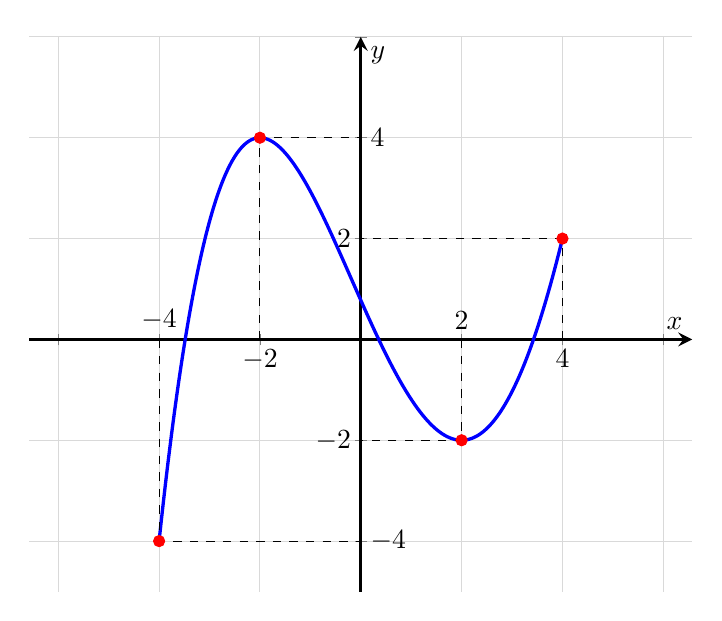
\begin{tikzpicture}[ 
    declare function={ 
    f(\x)=-(1/72)*\x^4+3/16*(\x^3)+(1/9)*\x^2-9/4*\x+7/9; 
    } 
    ]
    \begin{axis}[axis equal, 
    width=10 cm, 
    grid=major, 
    axis x line=middle, axis y line=middle, 
    axis line style = very thick, 
    grid style={gray!30}, 
    ymin=-5, ymax=6, yticklabels={}, ylabel=$y$, 
    xmin=-4, xmax=4, xticklabels={}, xlabel=$x$, 
    samples=500, 
    ] 
    \addplot[blue, very thick,domain=-4:4, smooth]{f(x)}; 
    \addplot [color=red, mark=*,only marks,samples at={-4,-2,2,4}] {f(x)}; 
    \pgfplotsinvokeforeach{-4,-2,2,4}{\draw[dashed] ({#1},0) |- (0,{f(#1)}); }
    \foreach \X/\Y in {-4/right,-2/left,2/left,4/right} 
    {\edef\temp{\noexpand\node[\Y] at (0,\X) {$\X$};} 
    \temp}
    \foreach \X/\Y in {-4/above,-2/below,2/above,4/below} 
    {\edef\temp{\noexpand\node[\Y] at (\X,0) {$\X$};} 
        \temp} 
    \end{axis}
    \end{tikzpicture} \par
  \ans{
    \begin{tikzpicture}
      \tkzTabInit{$x$ / 1 , $f(x)$ / 2}{\textcolor{green}{$-4$}, \textcolor{red}{$-2$}, $2$, $4$}
      \tkzTabVar{-/ \textcolor{green}{$-4$}, +/\textcolor{red}{$4$}, -/$-2$, +/$2$}
   \end{tikzpicture}
   \begin{itemize}
    \item[$\bullet$] \textcolor{red}{4} est le maximum de \(f\) sur l'intervalle \([-4; 4]\). Il est atteint en \textcolor{red}{\(x=-2\)})
    \item[$\bullet$] \textcolor{green}{-4} est le minimum de \(f\) sur l'intervalle \([-4; 4]\). Il est atteint en \textcolor{red}{\(x=-4\)})
   \end{itemize}
  }{5}{FALSE}

  \item Représenter le tableau de variation de la fonction carré. \par
  \ans{
    \begin{tikzpicture}
      \tkzTabInit{$x$ / 1 , \(x^2\) / 2}{$-\infty$,$0$, $+\infty$}
      \tkzTabVar{+/$+\infty$,-/$0$,+/$+\infty$}
   \end{tikzpicture}
  }{5}{FALSE}
  \item Représenter le tableau de variation de la fonction inverse. \par
    \ans{
      \begin{tikzpicture}
        \tkzTabInit{$x$ /1,$\frac{1}{x} $ /3}{$-\infty$,$0$,$+\infty$}%
        \tkzTabVar{+/ $0$ / ,-D+/ $-\infty$ / $+\infty$ , -/ $0$ /}
        \end{tikzpicture}
  }{5}{FALSE}
  \item Représenter le tableau de variation de la fonction racine carrée. \par
  \ans{
  \begin{tikzpicture}
  \tkzTabInit{$x$ /1,$\sqrt{x}$ /2}{$0$, $+\infty$}
  \tkzTabVar{- / 0, + / $+\infty$}%
  \end{tikzpicture}
  }{5}{FALSE}
  \item Représenter le tableau de variation de la fonction cube. \par
  \ans{
    \begin{tikzpicture}
      \tkzTabInit{$x$ /1,$x^3$ /2}{$-\infty$, $+\infty$}
      \tkzTabVar{- / $-\infty$, + / $+\infty$}%
      \end{tikzpicture}
  }{5}{FALSE}
\end{enumerate}
\end{document}
